\documentclass[14pt,a4paper]{extarticle}
% =============================================================
% preamble_compact.tex — компактный вариант оформления отчётов
% Основа — preamble.tex (СТП БГУИР); здесь только уплотнение:
% разделы без принудительного перехода на новую страницу,
% меньшие вертикальные отступы, плотные списки и подписи.
% =============================================================
% =============================================================
% preamble.tex — Shared LaTeX preamble for genetic/evolutionary reports
% Conforming to BSUIR STP 01-2024
% =============================================================

% Encoding and language
\usepackage[utf8]{inputenc}
\usepackage[T2A]{fontenc}
\usepackage[russian]{babel}

% Times New Roman font
\usepackage{tempora}

% Page geometry: STP 2.1.1
\usepackage{geometry}
\geometry{left=30mm, right=15mm, top=20mm, bottom=20mm}

% Line spacing: STP 2.1.1
\usepackage{setspace}
\singlespacing

% Allow TeX a bit more flexibility to avoid overflow
\pretolerance=1000
\tolerance=2000
\emergencystretch=3em

% Paragraph indent
\usepackage{indentfirst}
\setlength{\parindent}{1.25cm}

% Page numbers
\usepackage{fancyhdr}
\pagestyle{fancy}
\fancyhf{}
\fancyfoot[R]{\thepage}
\renewcommand{\headrulewidth}{0pt}
\fancypagestyle{plain}{%
  \fancyhf{}%
  \fancyfoot[R]{\thepage}%
  \renewcommand{\headrulewidth}{0pt}%
}

% Math
\usepackage{amsmath,amssymb}

% Graphics
\usepackage{graphicx}
\usepackage{float}
\usepackage{xcolor}

% Tables
\usepackage{booktabs}
\usepackage{tabularx}
\usepackage{multirow}
\usepackage{longtable}

% Captions
\usepackage{caption}
\captionsetup[figure]{
  labelsep=endash,
  justification=centering,
  font={normalsize},
  name=Рисунок
}
\captionsetup[table]{
  labelsep=endash,
  justification=raggedright,
  singlelinecheck=false,
  font={normalsize},
  name=Таблица
}

% Section formatting
\usepackage{titlesec}
\titleformat{\section}
  {\newpage\normalfont\fontsize{14}{18}\selectfont\bfseries}
  {\thesection}{0.5em}{\MakeUppercase}
\titlespacing*{\section}{1.25cm}{0pt}{14pt}

\titleformat{\subsection}
  {\normalfont\fontsize{14}{18}\selectfont\bfseries}
  {\thesubsection}{0.5em}{}
\titlespacing*{\subsection}{1.25cm}{14pt}{14pt}

\titleformat{\subsubsection}
  {\normalfont\fontsize{14}{18}\selectfont\bfseries}
  {\thesubsubsection}{0.5em}{}
\titlespacing*{\subsubsection}{1.25cm}{14pt}{14pt}

% Unnumbered sections
\newcommand{\sectioncenter}[1]{%
  \newpage
  \phantomsection
  \addcontentsline{toc}{section}{#1}
  \begin{center}
    \textbf{\MakeUppercase{#1}}
  \end{center}
  \vspace{14pt}
}

% Table of contents formatting
\usepackage{tocloft}
\renewcommand{\cftsecfont}{\normalfont}
\renewcommand{\cftsecpagefont}{\normalfont}
\renewcommand{\cftsubsecfont}{\normalfont}
\renewcommand{\cftsubsecpagefont}{\normalfont}
\renewcommand{\cftsecleader}{\cftdotfill{\cftdotsep}}
\renewcommand{\cftdotsep}{1}
\renewcommand{\contentsname}{\hfill\textbf{СОДЕРЖАНИЕ}\hfill}
\renewcommand{\cftaftertoctitle}{\hfill}

% Lists
\usepackage{enumitem}
\setlist[itemize]{noitemsep, topsep=0pt, leftmargin=1.25cm, label=--}
\setlist[enumerate]{noitemsep, topsep=0pt, leftmargin=1.25cm}

% Code listings
\usepackage{listings}
\usepackage{fancyvrb}
\lstset{
  basicstyle=\ttfamily\small,
  frame=single,
  breaklines=true,
  showstringspaces=false,
  inputencoding=utf8,
  extendedchars=true,
  literate={а}{{\cyra}}1 {б}{{\cyrb}}1 {в}{{\cyrv}}1 {г}{{\cyrg}}1
           {д}{{\cyrd}}1 {е}{{\cyre}}1 {ж}{{\cyrzh}}1 {з}{{\cyrz}}1
           {и}{{\cyri}}1 {й}{{\cyrishrt}}1 {к}{{\cyrk}}1 {л}{{\cyrl}}1
           {м}{{\cyrm}}1 {н}{{\cyrn}}1 {о}{{\cyro}}1 {п}{{\cyrp}}1
           {р}{{\cyrr}}1 {с}{{\cyrs}}1 {т}{{\cyrt}}1 {у}{{\cyru}}1
           {ф}{{\cyrf}}1 {х}{{\cyrh}}1 {ц}{{\cyrc}}1 {ч}{{\cyrch}}1
           {ш}{{\cyrsh}}1 {щ}{{\cyrshch}}1 {ъ}{{\cyrhrdsn}}1
           {ы}{{\cyrery}}1 {ь}{{\cyrsftsn}}1 {э}{{\cyrerev}}1
           {ю}{{\cyryu}}1 {я}{{\cyrya}}1
}

% Hyperlinks
\usepackage{hyperref}
\hypersetup{
  colorlinks=true,
  linkcolor=black,
  urlcolor=blue,
  citecolor=black,
}

% Number figures and tables within sections
\numberwithin{figure}{section}
\numberwithin{table}{section}
\numberwithin{equation}{section}

% Standard title page macro
\newcommand{\makegeclabtitle}[2]{%
  \begin{titlepage}
  \thispagestyle{empty}
  \begin{center}

  МИНИСТЕРСТВО ОБРАЗОВАНИЯ РЕСПУБЛИКИ БЕЛАРУСЬ

  \vspace{0.5em}

  Учреждение образования

  \vspace{0.5em}

  \textbf{<<Белорусский государственный университет информатики и радиоэлектроники>>}

  \vspace{2em}

  Факультет компьютерных систем и сетей

  \vspace{0.5em}

  Кафедра программного обеспечения информационных технологий

  \end{center}

  \vspace{3em}

  \begin{center}
  \textbf{ОТЧЕТ}

  \vspace{0.5em}

  по лабораторной работе №#1

  \vspace{0.5em}

  по дисциплине

  \vspace{0.5em}

  <<Генетические и эволюционные вычисления>>

  \vspace{0.5em}

  <<#2>>
  \end{center}

  \vspace{5em}

  \begin{flushright}
  \begin{minipage}{0.5\textwidth}
  \textbf{Выполнил:}\\
  Лебедевич Артем Владимирович\\
  магистрант группы 556301

  \vspace{0.6em}

  \textbf{Преподаватель:}\\
  Нестеренков Сергей Николаевич\\
  кандидат технических наук\\
  доцент кафедры ПОИТ
  \end{minipage}
  \end{flushright}

  \vfill

  \begin{center}
  Минск, 2026~г.
  \end{center}

  \end{titlepage}
}


% Разделы идут подряд, без \newpage
\titleformat{\section}
  {\normalfont\fontsize{14}{17}\selectfont\bfseries}
  {\thesection}{0.5em}{\MakeUppercase}
\titlespacing*{\section}{1.25cm}{12pt}{6pt}
\titlespacing*{\subsection}{1.25cm}{8pt}{4pt}

% Плотнее плавающие объекты и подписи
\setlength{\textfloatsep}{8pt plus 2pt minus 2pt}
\setlength{\floatsep}{6pt plus 2pt minus 2pt}
\setlength{\intextsep}{6pt plus 2pt minus 2pt}
\captionsetup[figure]{skip=3pt, font={small}}
\captionsetup[table]{skip=2pt, font={small}}
\setlength{\abovedisplayskip}{4pt}
\setlength{\belowdisplayskip}{4pt}

% Таблицы компактнее
\renewcommand{\arraystretch}{1.05}
\setlength{\tabcolsep}{5pt}

% Номера рисунков и таблиц — сквозные (без привязки к разделам)
\counterwithout{figure}{section}
\counterwithout{table}{section}
\counterwithout{equation}{section}

\graphicspath{{figures/}}

\begin{document}

\makegeclabtitle{5}{Поиск экстремума функции одной переменной с помощью генетического алгоритма с бинарным представлением особей}

\section{Цель работы}

Изучить основные понятия теории генетических алгоритмов (ГА), реализовать классический простой ГА с представлением решений в форме бинарных строк и исследовать влияние его параметров на качество и надёжность поиска. Вариант~3: найти максимум функции
\begin{equation}
f(t) = (t - 1{,}3)\sin(0{,}5\pi t + 1), \qquad t \in [0;\ 7].
\end{equation}

\section{Краткие теоретические сведения}

\textbf{Кодирование.} Число $t \in [a;\ b]$ представляется строкой $s$ из $L$ бит: $t = a + \mathrm{dec}(s)\,(b - a)/(2^L - 1)$, точность представления $\Delta = (b - a)/(2^L - 1)$.

\textbf{Простой ГА} повторяет цикл: оценка приспособленности $\to$ селекция $\to$ кроссинговер $\to$ мутация. Пропорциональная селекция (рулетка) выбирает особь с вероятностью $p_i = f'_i / \sum_j f'_j$, где $f'_i = f_i - \min f + \varepsilon$ (сдвиг нужен, так как $f$ принимает отрицательные значения). Одноточечный кроссинговер с вероятностью $P_c$ обменивает части двух хромосом после случайной точки разреза. Побитовая мутация инвертирует каждый бит с вероятностью $P_m$. Элитизм переносит лучшую найденную особь в следующее поколение.

\section{Ход работы}

\textbf{Эталон.} Численный поиск (сетка из 700\,001 точки и метод Брента) даёт глобальный максимум $t^* = 4{,}488826$, $f(t^*) = 3{,}127117$. Функция имеет ещё один, незначительный, локальный максимум $f(1{,}332) = 0{,}002$.

\textbf{Реализация.} ГА реализован на NumPy (\texttt{lab\_05.ipynb}) с векторизованными операторами. Параметры по умолчанию: $N = 60$, $L = 20$ ($\Delta = 6{,}7 \cdot 10^{-6}$), $P_c = 0{,}85$, $P_m = 0{,}01$, 200 поколений, элитизм. Запуск считается успешным, если найдено решение с $|t - t^*| < 10^{-3}$.

\begin{table}[H]
\caption{Результат поиска максимума (N = 60, L = 20, $P_c = 0{,}85$, $P_m = 0{,}01$)}
\label{tab:result}
\centering
\small
\begin{tabular}{lc}
\toprule
Параметр & Значение \\
\midrule
$t^*$ (эталон) & 4.488826 \\
$f(t^*)$ (эталон) & 3.127117 \\
$t$ (ГА) & 4.488825 \\
$f(t)$ (ГА) & 3.127117 \\
$|t - t^*|$ & 9.2e-07 \\
Поколение попадания & 7 \\
Успешных запусков из 50 & 47 \\
Поколений до попадания (медиана / макс.) & 11 / 168 \\
\bottomrule
\end{tabular}
\end{table}


Результат основного запуска и статистика по 50 запускам приведены в таблице~\ref{tab:result}, динамика~--- на рисунках~\ref{fig:pop} и~\ref{fig:conv}. Уже к 10-му поколению популяция собирается у глобального максимума; средняя приспособленность отстаёт от лучшей из-за мутаций.

\begin{figure}[H]
\centering
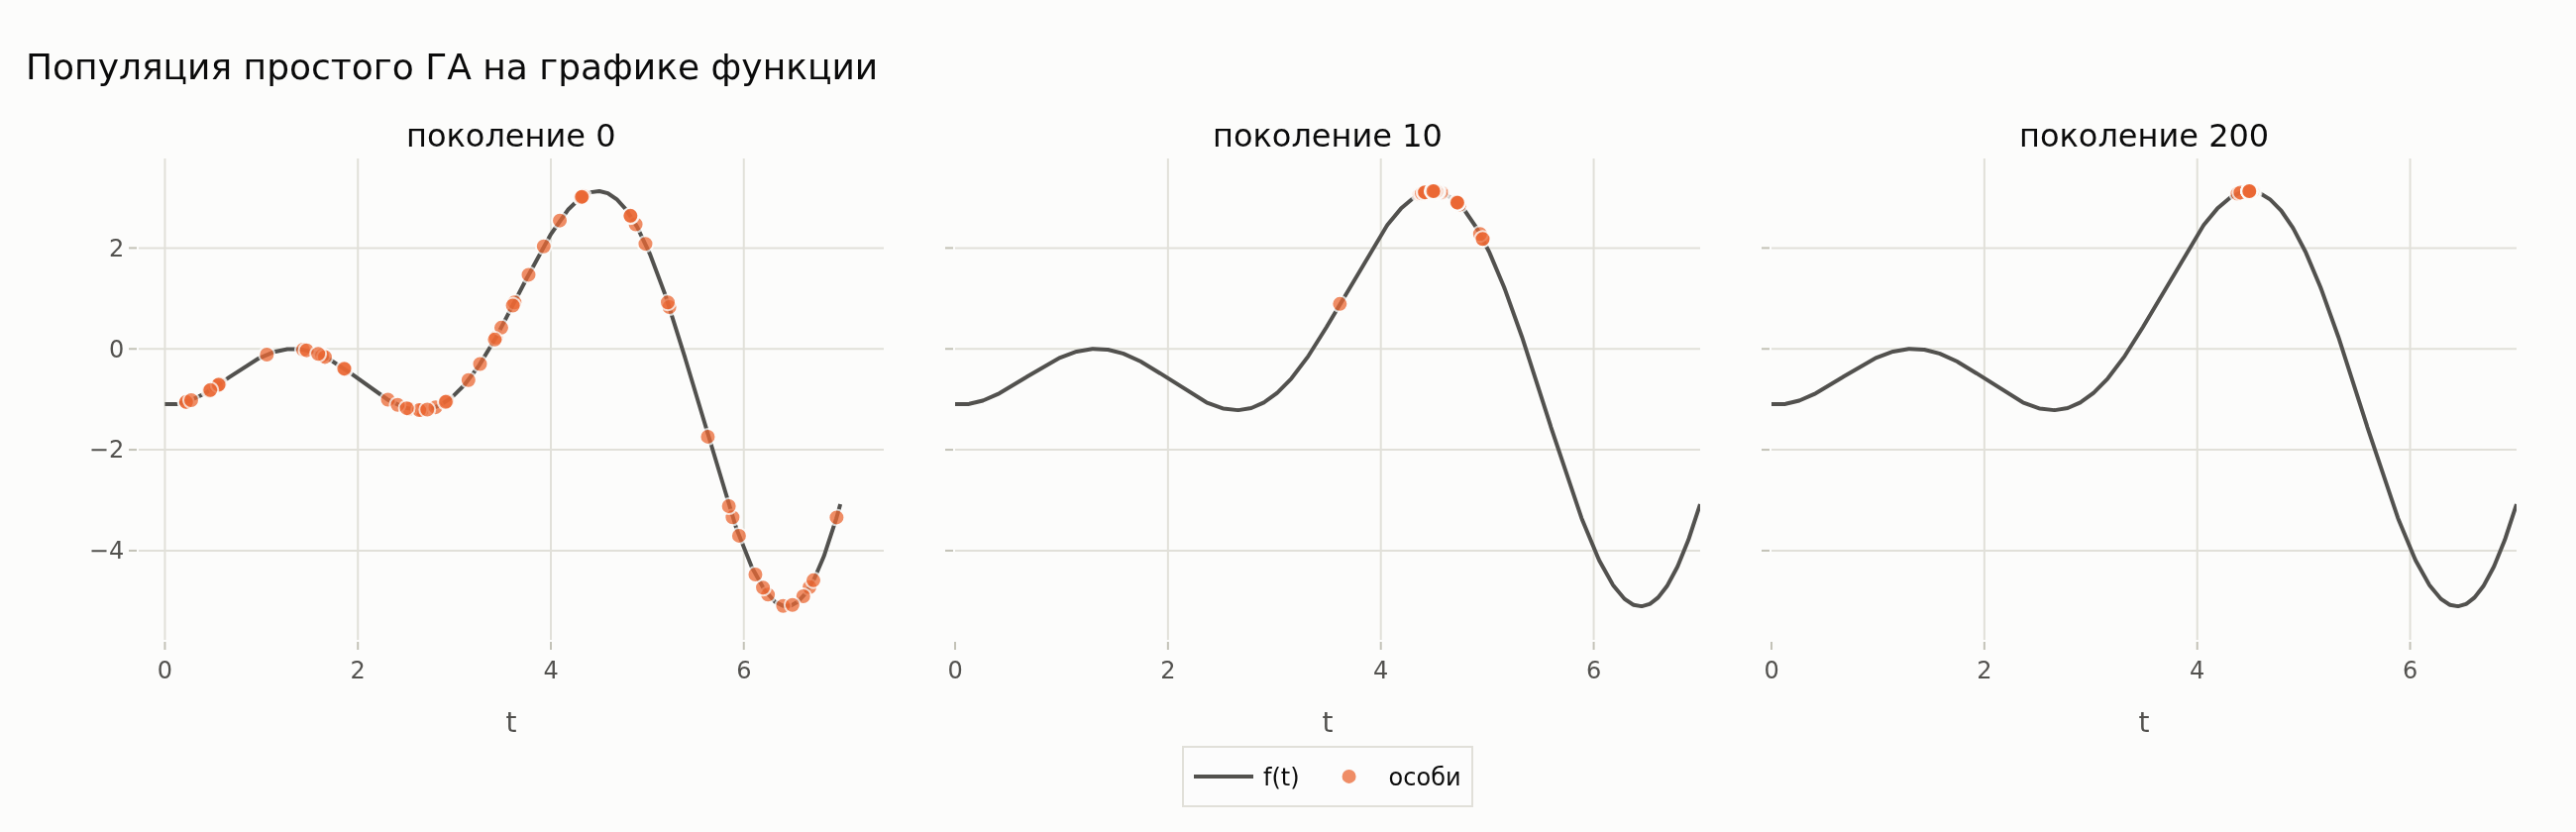
\includegraphics[width=\textwidth]{03_population.png}
\caption{Популяция на графике функции: поколения 0, 10 и 200}
\label{fig:pop}
\end{figure}

\begin{figure}[H]
\centering
\begin{minipage}{0.49\textwidth}\centering
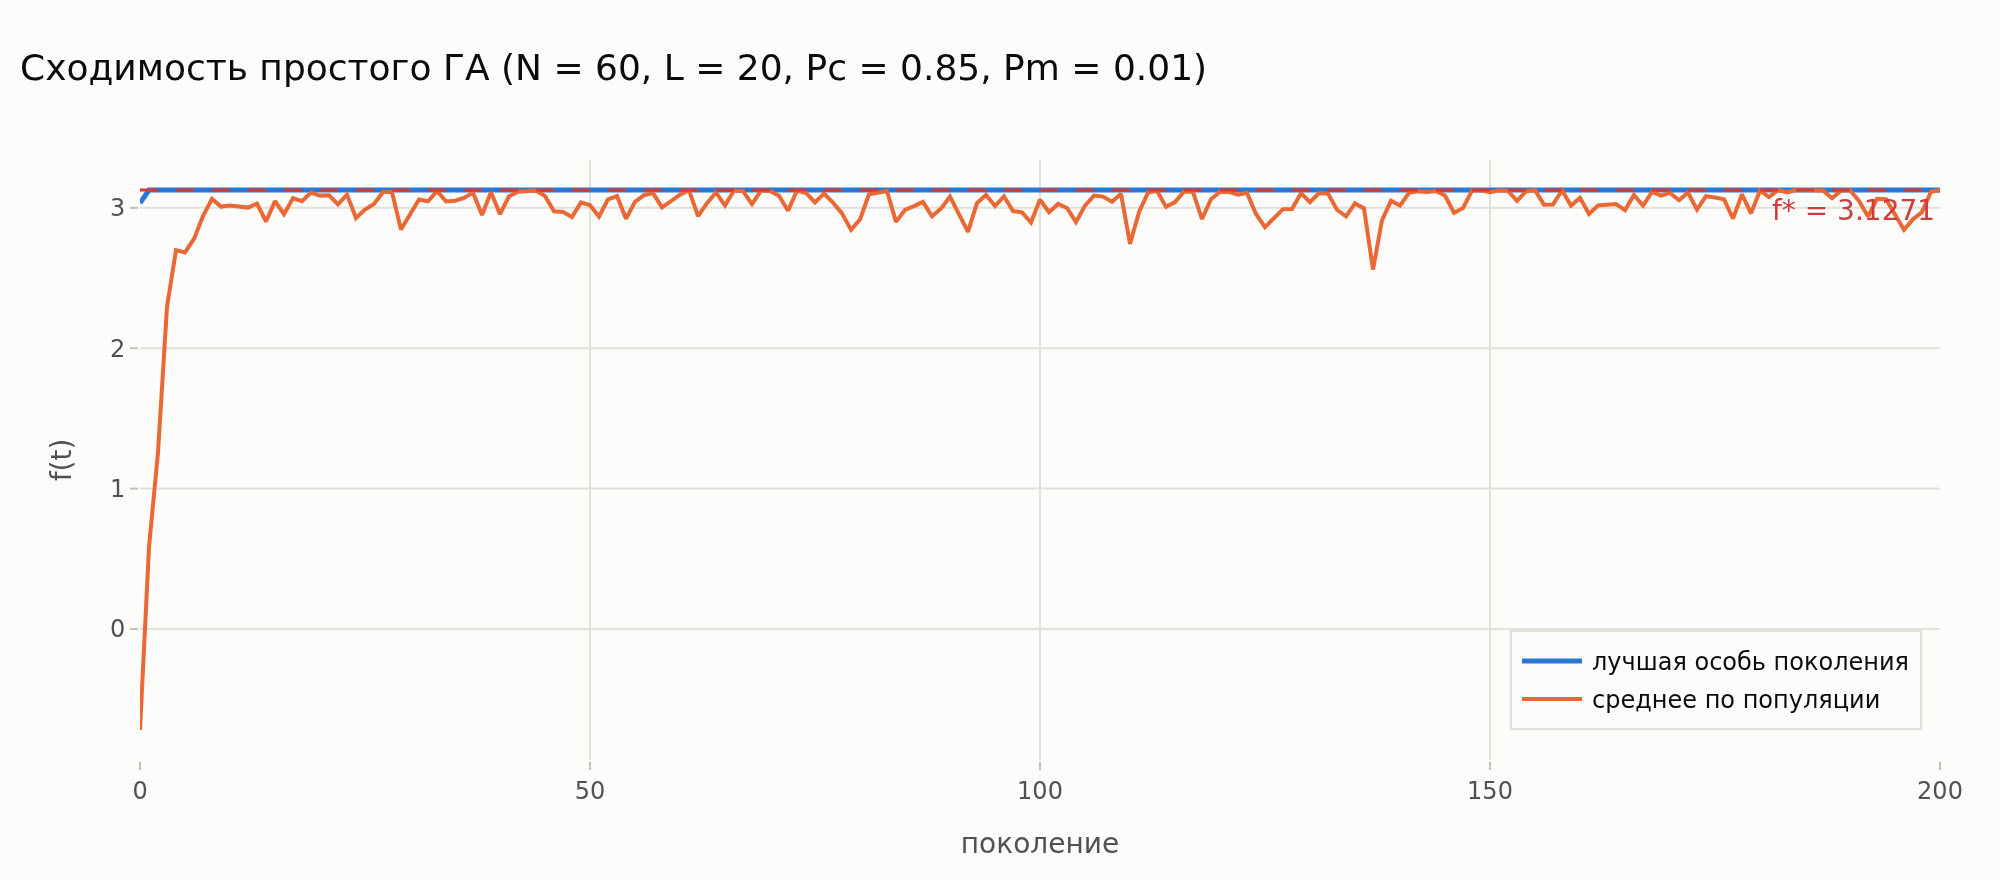
\includegraphics[width=\textwidth]{02_convergence.png}
\end{minipage}\hfill
\begin{minipage}{0.49\textwidth}\centering
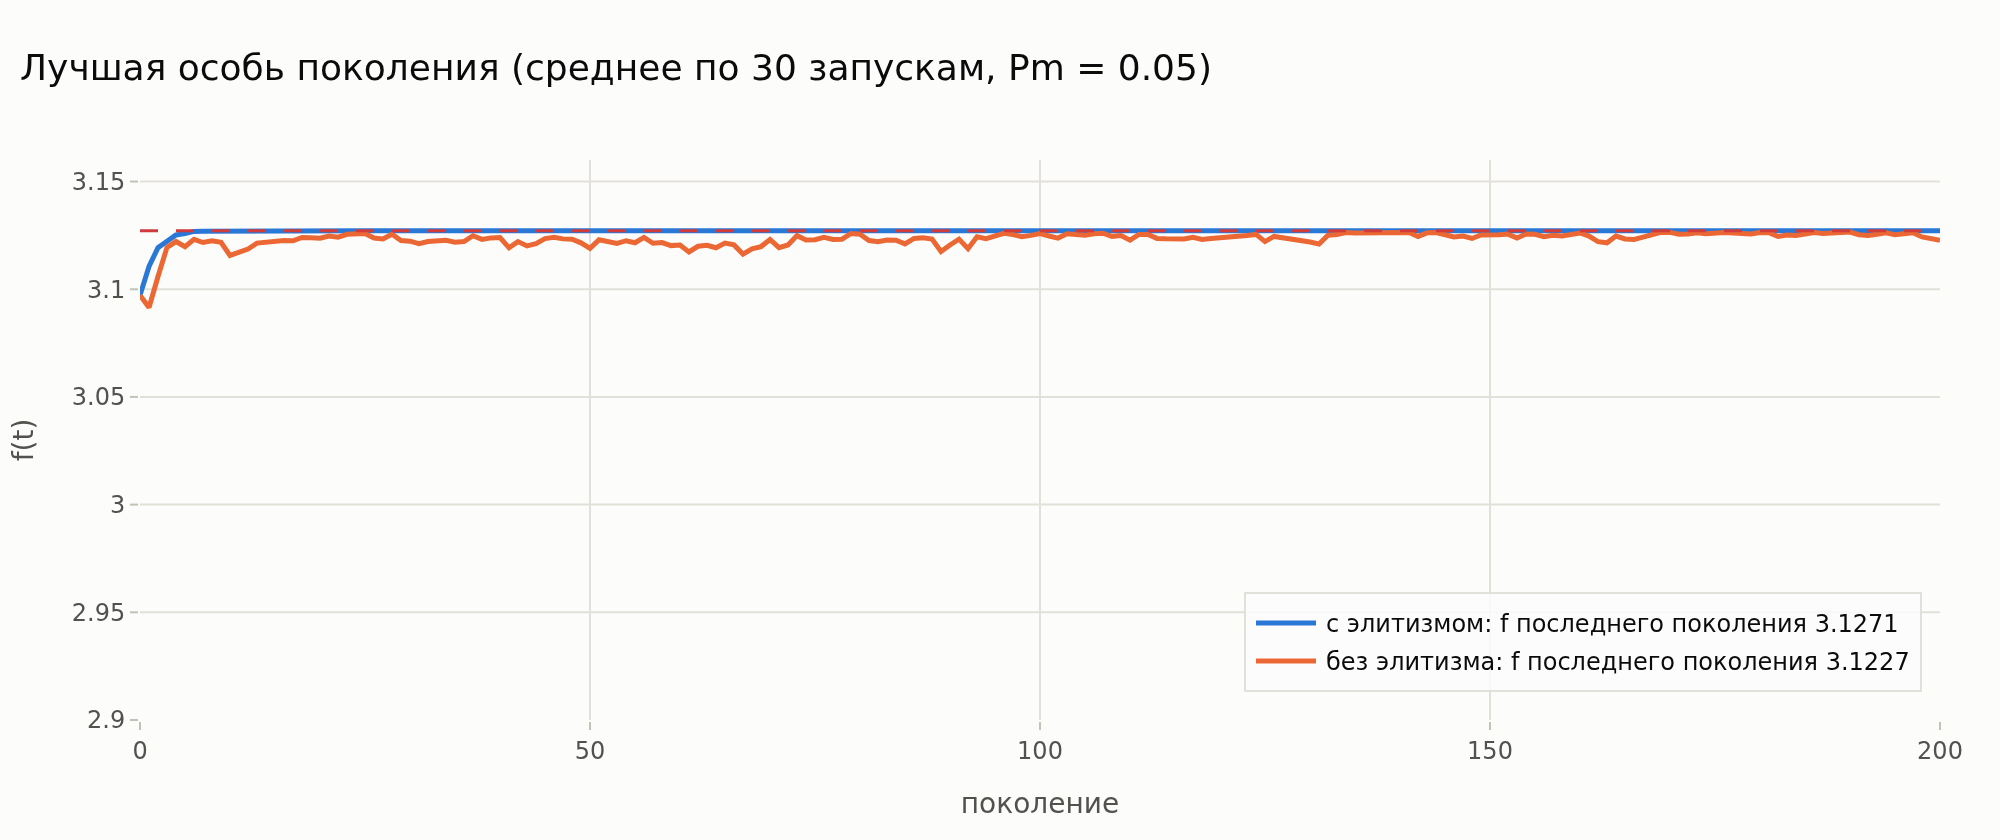
\includegraphics[width=\textwidth]{05_elitism.png}
\end{minipage}
\caption{Слева~--- сходимость основного запуска; справа~--- лучшая особь поколения с элитизмом и без (среднее по 30 запускам, $P_m = 0{,}05$)}
\label{fig:conv}
\end{figure}

\textbf{Исследование параметров.} Каждый параметр менялся при фиксированных остальных, по 30 запусков на значение (таблица~\ref{tab:params}, рисунок~\ref{fig:params}).

\begin{figure}[H]
\centering
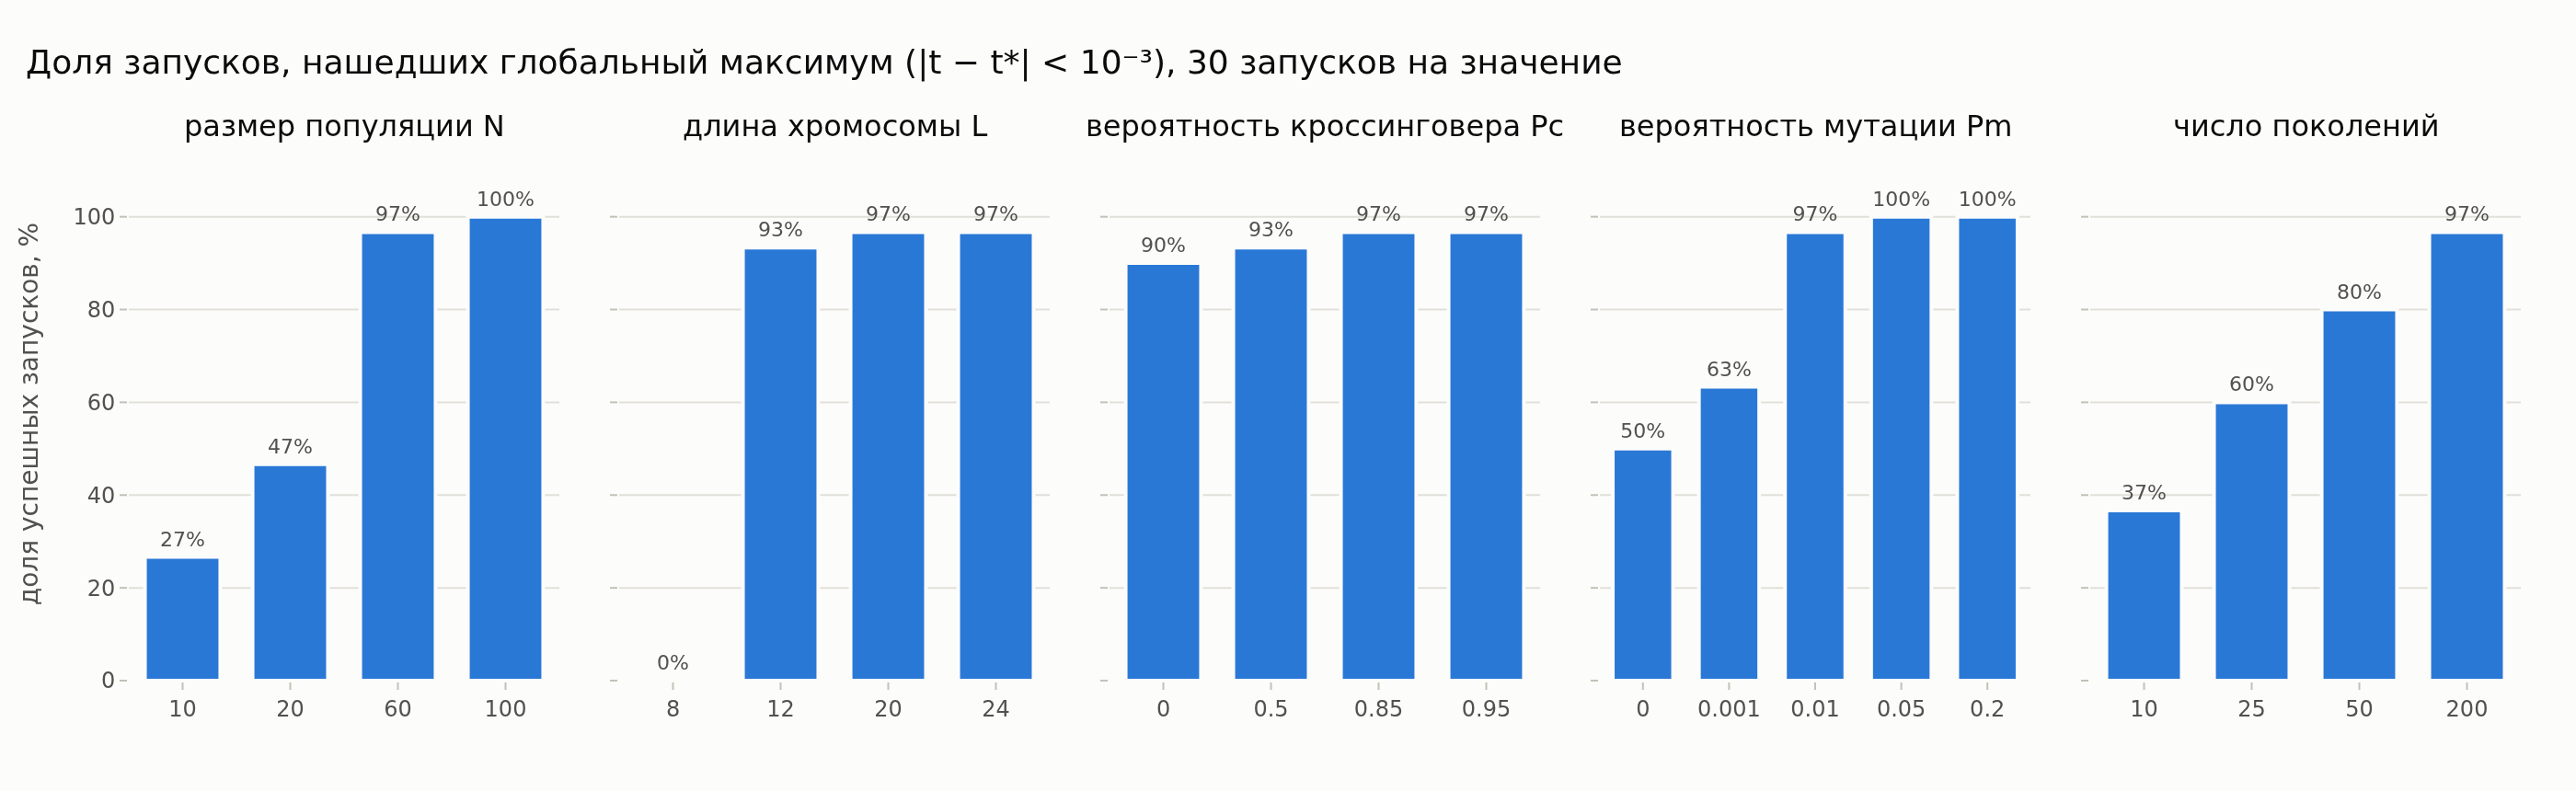
\includegraphics[width=\textwidth]{04_parameters.png}
\caption{Доля успешных запусков при варьировании параметров}
\label{fig:params}
\end{figure}

\begin{table}[H]
\caption{Влияние параметров ГА (30 запусков на значение)}
\label{tab:params}
\centering
\small
\begin{tabular}{lccccc}
\toprule
Параметр & Значение & Успехов, \% & Среднее $f$ & Худшее $f$ & Поколений \\
\midrule
размер популяции N & 10 & 27 & 3.1082 & 3.0745 & 60 \\
размер популяции N & 20 & 47 & 3.1218 & 3.0745 & 16 \\
размер популяции N & 60 & 97 & 3.1271 & 3.1270 & 15 \\
размер популяции N & 100 & 100 & 3.1271 & 3.1271 & 12 \\
длина хромосомы L & 8 & 0 & 3.1264 & 3.1264 & --- \\
длина хромосомы L & 12 & 93 & 3.1253 & 3.0739 & 11 \\
длина хромосомы L & 20 & 97 & 3.1271 & 3.1270 & 15 \\
длина хромосомы L & 24 & 97 & 3.1254 & 3.0745 & 16 \\
вероятность $P_c$ & 0 & 90 & 3.1271 & 3.1270 & 24 \\
вероятность $P_c$ & 0.5 & 93 & 3.1271 & 3.1270 & 17 \\
вероятность $P_c$ & 0.85 & 97 & 3.1271 & 3.1270 & 15 \\
вероятность $P_c$ & 0.95 & 97 & 3.1271 & 3.1270 & 12 \\
вероятность $P_m$ & 0 & 50 & 3.1270 & 3.1247 & 10 \\
вероятность $P_m$ & 0.001 & 63 & 3.1271 & 3.1270 & 8 \\
вероятность $P_m$ & 0.01 & 97 & 3.1271 & 3.1270 & 15 \\
вероятность $P_m$ & 0.05 & 100 & 3.1271 & 3.1271 & 13 \\
вероятность $P_m$ & 0.2 & 100 & 3.1271 & 3.1271 & 18 \\
число поколений & 10 & 37 & 3.1270 & 3.1266 & 4 \\
число поколений & 25 & 60 & 3.1271 & 3.1270 & 10 \\
число поколений & 50 & 80 & 3.1271 & 3.1270 & 11 \\
число поколений & 200 & 97 & 3.1271 & 3.1270 & 15 \\
\bottomrule
\end{tabular}
\end{table}


\section{Выводы}

\begin{enumerate}
\item Простой ГА находит глобальный максимум $t^* = 4{,}48883$, $f^* = 3{,}12712$ с погрешностью $9 \cdot 10^{-7}$~--- на уровне точности 20-битного кода. Окрестность $10^{-3}$ достигается на 7-м поколении (около 420 вычислений функции).
\item Из 50 запусков 47 успешны, медиана~--- 11 поколений. Три неудачи~--- не ложный максимум, а остановка на плоской вершине ($f = 3{,}1270$ при $|t - t^*| > 10^{-3}$). Вблизи вершины значения $f$ почти равны, рулетка теряет давление отбора, и доводку выполняет только мутация.
\item Размер популяции~--- главный фактор надёжности: 27\,\% успехов при $N = 10$, 97\,\% при $N = 60$, 100\,\% при $N = 100$.
\item Длина хромосомы ограничивает точность: при $L = 8$ шаг $0{,}027$ больше допуска, и попадание невозможно в принципе. Рост $L$ с 20 до 24 бит точность не повышает, а пространство поиска увеличивает в 16 раз.
\item Мутация необходима: при $P_m = 0$ популяция вырождается (50\,\% успехов), при $P_m = 0{,}05$--$0{,}2$ успех стопроцентный. Кроссинговер ускоряет поиск (медиана 24 поколения при $P_c = 0$ и 12 при $P_c = 0{,}95$).
\item Элитизм обеспечивает монотонный рост лучшего решения: без него найденный максимум теряется из-за мутаций, и лучшая особь последнего поколения хуже ($f = 3{,}1227$ против $3{,}1271$).
\end{enumerate}


\end{document}
